\documentclass[11pt,preprint, authoryear]{elsarticle}

\usepackage{lmodern}
%%%% My spacing
\usepackage{setspace}
\setstretch{1.2}
\DeclareMathSizes{12}{14}{10}{10}

% Wrap around which gives all figures included the [H] command, or places it "here". This can be tedious to code in Rmarkdown.
\usepackage{float}
\let\origfigure\figure
\let\endorigfigure\endfigure
\renewenvironment{figure}[1][2] {
    \expandafter\origfigure\expandafter[H]
} {
    \endorigfigure
}

\let\origtable\table
\let\endorigtable\endtable
\renewenvironment{table}[1][2] {
    \expandafter\origtable\expandafter[H]
} {
    \endorigtable
}


\usepackage{ifxetex,ifluatex}
\usepackage{fixltx2e} % provides \textsubscript
\ifnum 0\ifxetex 1\fi\ifluatex 1\fi=0 % if pdftex
  \usepackage[T1]{fontenc}
  \usepackage[utf8]{inputenc}
\else % if luatex or xelatex
  \ifxetex
    \usepackage{mathspec}
    \usepackage{xltxtra,xunicode}
  \else
    \usepackage{fontspec}
  \fi
  \defaultfontfeatures{Mapping=tex-text,Scale=MatchLowercase}
  \newcommand{\euro}{€}
\fi

\usepackage{amssymb, amsmath, amsthm, amsfonts}

\def\bibsection{\section*{References}} %%% Make "References" appear before bibliography


\usepackage[round]{natbib}

\usepackage{longtable}
\usepackage[margin=2.3cm,bottom=2cm,top=2.5cm, includefoot]{geometry}
\usepackage{fancyhdr}
\usepackage[bottom, hang, flushmargin]{footmisc}
\usepackage{graphicx}
\numberwithin{equation}{section}
\numberwithin{figure}{section}
\numberwithin{table}{section}
\setlength{\parindent}{0cm}
\setlength{\parskip}{1.3ex plus 0.5ex minus 0.3ex}
\usepackage{textcomp}
\renewcommand{\headrulewidth}{0.2pt}
\renewcommand{\footrulewidth}{0.3pt}

\usepackage{array}
\newcolumntype{x}[1]{>{\centering\arraybackslash\hspace{0pt}}p{#1}}

%%%%  Remove the "preprint submitted to" part. Don't worry about this either, it just looks better without it:
\makeatletter
\def\ps@pprintTitle{%
  \let\@oddhead\@empty
  \let\@evenhead\@empty
  \let\@oddfoot\@empty
  \let\@evenfoot\@oddfoot
}
\makeatother

 \def\tightlist{} % This allows for subbullets!

\usepackage{hyperref}
\hypersetup{breaklinks=true,
            bookmarks=true,
            colorlinks=true,
            citecolor=blue,
            urlcolor=blue,
            linkcolor=blue,
            pdfborder={0 0 0}}


% The following packages allow huxtable to work:
\usepackage{siunitx}
\usepackage{multirow}
\usepackage{hhline}
\usepackage{calc}
\usepackage{tabularx}
\usepackage{booktabs}
\usepackage{caption}


\newenvironment{columns}[1][]{}{}

\newenvironment{column}[1]{\begin{minipage}{#1}\ignorespaces}{%
\end{minipage}
\ifhmode\unskip\fi
\aftergroup\useignorespacesandallpars}

\def\useignorespacesandallpars#1\ignorespaces\fi{%
#1\fi\ignorespacesandallpars}

\makeatletter
\def\ignorespacesandallpars{%
  \@ifnextchar\par
    {\expandafter\ignorespacesandallpars\@gobble}%
    {}%
}
\makeatother

\newlength{\cslhangindent}
\setlength{\cslhangindent}{1.5em}
\newenvironment{CSLReferences}%
  {\setlength{\parindent}{0pt}%
  \everypar{\setlength{\hangindent}{\cslhangindent}}\ignorespaces}%
  {\par}


\urlstyle{same}  % don't use monospace font for urls
\setlength{\parindent}{0pt}
\setlength{\parskip}{6pt plus 2pt minus 1pt}
\setlength{\emergencystretch}{3em}  % prevent overfull lines
\setcounter{secnumdepth}{5}

%%% Use protect on footnotes to avoid problems with footnotes in titles
\let\rmarkdownfootnote\footnote%
\def\footnote{\protect\rmarkdownfootnote}
\IfFileExists{upquote.sty}{\usepackage{upquote}}{}

%%% Include extra packages specified by user

%%% Hard setting column skips for reports - this ensures greater consistency and control over the length settings in the document.
%% page layout
%% paragraphs
\setlength{\baselineskip}{12pt plus 0pt minus 0pt}
\setlength{\parskip}{12pt plus 0pt minus 0pt}
\setlength{\parindent}{0pt plus 0pt minus 0pt}
%% floats
\setlength{\floatsep}{12pt plus 0 pt minus 0pt}
\setlength{\textfloatsep}{20pt plus 0pt minus 0pt}
\setlength{\intextsep}{14pt plus 0pt minus 0pt}
\setlength{\dbltextfloatsep}{20pt plus 0pt minus 0pt}
\setlength{\dblfloatsep}{14pt plus 0pt minus 0pt}
%% maths
\setlength{\abovedisplayskip}{12pt plus 0pt minus 0pt}
\setlength{\belowdisplayskip}{12pt plus 0pt minus 0pt}
%% lists
\setlength{\topsep}{10pt plus 0pt minus 0pt}
\setlength{\partopsep}{3pt plus 0pt minus 0pt}
\setlength{\itemsep}{5pt plus 0pt minus 0pt}
\setlength{\labelsep}{8mm plus 0mm minus 0mm}
\setlength{\parsep}{\the\parskip}
\setlength{\listparindent}{\the\parindent}
%% verbatim
\setlength{\fboxsep}{5pt plus 0pt minus 0pt}



\begin{document}



\begin{frontmatter}  %

\title{Predicting Loan Defaults}

% Set to FALSE if wanting to remove title (for submission)




\author[Add1]{Zander Prinsloo\footnote{\textbf{Contributions:} Thank you
  to Zhou Xu for providing the raw data and a description of the data
  tables on GitHub at \url{https://github.com/zhouxu-ds} \newline \_\_}}
\ead{20065124@sun.ac.za}





\address[Add1]{Stellenbosch University, South Africa}

\cortext[cor]{Corresponding author: Zander Prinsloo\footnote{\textbf{Contributions:}
  Thank you to Zhou Xu for providing the raw data and a description of
  the data tables on GitHub at \url{https://github.com/zhouxu-ds}
  \newline \_\_}}

\begin{abstract}
\small{
This project analysis loan defaults. Using anonymized financial data
containing client and district-level informatino from a Czech bank, the
loan repayment information of clients can be analysed. Thorough
exploratory data analysis informs the feature selection and modeling
approaches. Logistic regression, a common approach for credit-risk
screening, is compared to XGBoost in predicting loan defaults. It is
found that the optimal regularised logistic regression model performs
comparably to the fully tuned XGBoost approach. Thereafter, a causal
forest is utilised to investigate the effect of entrepreneurship in
districts on loan defaults. It is found that a high density of
entrepreneurs has a positive effect on loan default rates, but that
there is substantial heterogeneity and non-linearity in these treatment
effects, justifying the flexible machine learning approach.
}
\end{abstract}

\vspace{1cm}

\begin{keyword}
\footnotesize{
Loan Defaults \sep Penalized Logistic Regression \sep XGBoost
\sep Causal Forest \\ \vspace{0.3cm}
\textit{JEL classification} \sep 
}
\end{keyword}
\vspace{0.5cm}
\end{frontmatter}



%________________________
% Header and Footers
%%%%%%%%%%%%%%%%%%%%%%%%%%%%%%%%%
\pagestyle{fancy}
\chead{}
\rhead{}
\lfoot{}
\rfoot{\footnotesize Page \thepage}
\lhead{}
%\rfoot{\footnotesize Page \thepage } % "e.g. Page 2"
\cfoot{}

%\setlength\headheight{30pt}
%%%%%%%%%%%%%%%%%%%%%%%%%%%%%%%%%
%________________________

\headsep 35pt % So that header does not go over title




\hypertarget{introduction}{%
\section{\texorpdfstring{Introduction
\label{Introduction}}{Introduction }}\label{introduction}}

The aim of this project is to analyse and predict loan defaults of
banking clients in Czech Republic in 1999. This would provide useful
information to banks in managing credit risk when granting loans. The
process of building prediction models starts with an initial, thorough
exploration of the data. The data sets are described, as well as the
process by which they are collated. Information on individual
transactions, loans, clients, districts in Czech, etc. are combined
through a series of unique identifiers to create one data set where the
unit of observation is the unique loan granted. This process of data
wrangling is made more efficient through the use of databases that exist
in memory and means that queries can be submitted more efficiently than
when working with the entire data frame as an object in R. After
collecting the collated and tidy data set, series of visualisations
informs further feature and target engineering decisions. This
exploratory data analysis is vital as it allows an understanding of the
data through visualisation, informing both the engineering of features
and targets and the modelling that comes thereafter. A binary variable,
\(Defaults\), becomes the target of the modeling.

Logistic regression is commonly used for credit-risk screening
\protect\hyperlink{ref-ESL}{Friedman, Hastie \& Tibshirani}
(\protect\hyperlink{ref-ESL}{2009}). The standard multiple logistic
regresssion model provides a good benchmark model for predicting loan
defaults. However, this model is too flexible, with the high variance
leading to a lower prediction accuracy. While dimension reduction
through principal component analysis does improve the prediction
accuracy slightly, the largest improvements are attained when
regularizing the logistic regression model. Decreasing variance by using
the penalised logistic regression model substantially improves
prediction accuracy. The logistic regression approach is compared to a
more state-of-the-art tree-based ensemble approach through using eXtreme
Gradient Boosting (XGBoost). Three variations of this model is
presented. While the default hyperparameters generally perform well
\protect\hyperlink{ref-Boehmke}{Boehmke \& Greenwell}
(\protect\hyperlink{ref-Boehmke}{2019}), a substantial improvement in
prediction accuracy is observed when conducting hyperparameter tuning.
Again, regularisation proves important. The fully tuned model has the
lowest cross-validation (CV) error rate, as is expected. However, the
final optimal XGBoost model has a very comparable CV error rate to the
penalized logistic regression estimator.

Finally, a causal forest approach is utilised to investigate the effect
of a high number of entrepreneurs in a district on loan default rates.
It is found that having a large number of entrepreneurs in a district
does increase the loan default risk, however, there is substantial
heterogeneity in this effect. Banks should closely monitor clients with
high average transactions that come from highly entrepreneurial district
as they may pose a large credit risk.

\hypertarget{data}{%
\section{\texorpdfstring{Data \label{Data}}{Data }}\label{data}}

This section discusses the data source, the cleaning and merging of data
sets, exploratory data analysis, and feature/target engineering. These
decisions are important in shaping the modelling decisions that follow.
Additionally, it allows an understanding of the data that aids in the
obejctive of the project, which is to analyse loan defaults.

\hypertarget{data-sources}{%
\subsection{Data Sources}\label{data-sources}}

This analysis is done on real, anonymized data from a Czech bank in
1999, released for the PKDD'99 Discovery Challenge
\protect\hyperlink{ref-Data}{Berka} (\protect\hyperlink{ref-Data}{1999})
. It provides information on clients, accounts, transactions, loans,
etc. This information is contained in 8 relational data sets, listed and
described briefly below:

\begin{enumerate}
\def\labelenumi{\arabic{enumi}.}
\tightlist
\item
  \emph{Relation Account}, where each record describes static
  characteristics of an account. It contains 4500 objects (rows) - one
  for each account
\item
  \emph{Relation Client}, where each observation describes
  characteristics of the client. It contains 5369 objects (rows) - one
  for each client.
\item
  \emph{Relation Disposition}, where each observation gives the
  relationship of a specific client to a specific account, i.e.~whether
  an owner of the account of not. It contains 4500 unique accounts and
  5369 unique clients.
\item
  \emph{Relation Permanent Order}, where each observation describes
  dynamic characteristics of a payment order. It contains 3758 unique
  accounts, and 6471 unique orders.
\item
  \emph{Relation Transaction}, describing much of the dynamic
  characteristics where each observation describes a transaction in an
  account. It contains 1056320 objects where each is a unique
  transaction. It also contains 4500 unique accounts.
\item
  \emph{Relation Loan}, where each observation describes a loan that has
  been granted for a specific account. It contains 682 observations,
  each being a unique loan attached to a unique account such that there
  are also 682 unique accounts in the data set.
\item
  \emph{Relation Credit Card}, where each observation describes a credit
  card issued to a particular account. It contains 892 rows where each
  row is a unique card that has been issued.
\item
  \emph{Relation Demographic}, where each observation describes the
  characteristics of a district. It contains 77 unique districts.
\end{enumerate}

Accounts have static and dynamic characteristics given in these tables.
The former include things like date of creation of the account, and the
latter is payments, total debited amounts, etc. that are updated over
time. This account information is combined with information on the
client that can manipulate the account, and demographic information
(such as unemployment rates, population size, urban ratio, etc.) on the
district where the client resides. Importantly, these accounts can also
be connected to specific loan information that will be analysed here.
These sources are combined to give a data set that is in terms of a loan
that is taken out by a unique account. The characteristics of the
account and client can then be used to predict whether or not a client
will default on the loan.

\hypertarget{data-cleaning}{%
\subsection{Data Cleaning}\label{data-cleaning}}

All data frames are housed as tables in the same DuckDB connection,
allowing a more efficient data cleaning and joining process before
collecting it as a data frame in the local R environment. This is useful
because the entire data set is not of interest. Rather, only a subset
that has been appropriately cleaned and transformed is used. For
example, the transaction data set alone has \emph{1 056 320} rows, one
for each transaction for each account, which would become
computationally expensive in wrangling. Therefore, a number of data
cleaning functions for each table are used, as well as a function to
merge the data into a final data set. The unique account, client, loan,
and district identifiers can be used to collate all the information into
one data set describing the characteristics of the client and unique
account that has taken out a loan.

An empty database connection, \texttt{con}, is opened using
\texttt{DBI::dbConnect()}. While this relies on SQL, the \texttt{dplyr}
package allows communication to the databases through the local R
environment. A \texttt{DuckDB} backend is enabled and it is specified as
a local connection existing in memory. The database tables that exist in
the connection are named df\_account, df\_card, df\_client, df\_disp,
df\_district, df\_loan, df\_order, df\_trans. The final merged data
table then includes 50 variables that will be analysed further below.

\hypertarget{exploratory-data-analysis}{%
\subsection{Exploratory Data Analysis}\label{exploratory-data-analysis}}

In this section further exploratory data analysis is conduced to develop
a better understanding of the characteristics and relationships between
features in the data set. This would inform further modeling and feature
engineering decisions to be made at a later stage.

\hypertarget{the-target-variable}{%
\subsubsection{The Target Variable}\label{the-target-variable}}

\begin{figure}[H]

{\centering 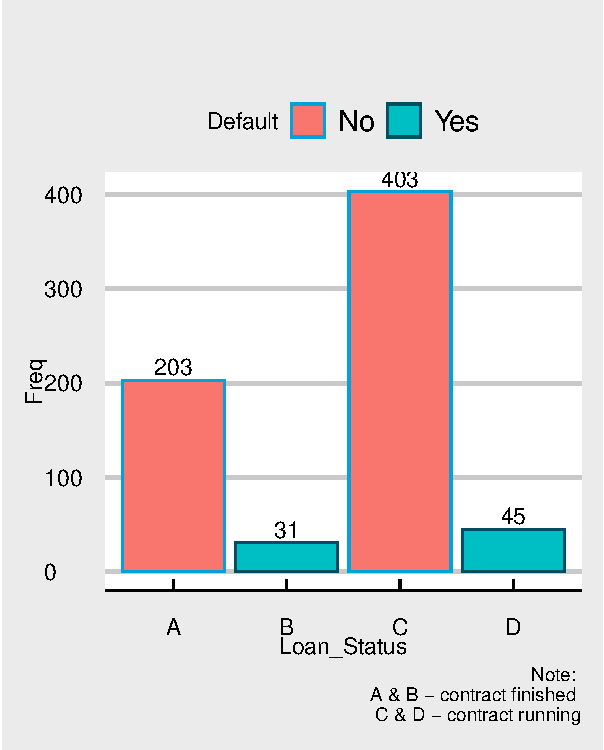
\includegraphics{DS-Report-20065124_files/figure-latex/FigureLoanStatus-1} 

}

\caption{Understanding Loan Statuses and Defaults \label{FigureLoanStatus}}\label{fig:FigureLoanStatus}
\end{figure}

\emph{Loan Status} is a variable given in the loans data table. It
classifies a loan into one of 4 classes, where A and C are not defaults
and B and D constitute defaults \protect\hyperlink{ref-Data}{Berka}
(\protect\hyperlink{ref-Data}{1999}). The distribution of loan status
shown in Figure \ref{FigureLoanStatus} indicates that there is a class
imbalance, where loans that are \emph{good} such that they are unlikely
to default (status A or C) are far more frequent than loans that are
defaulting on their payments (status B or D). It is important to
consider this class imbalance because an under-representation of one
class could lead to models performing badly and misunderstanding
relationships between features and loan defaults
\protect\hyperlink{ref-Boehmke}{Boehmke \& Greenwell}
(\protect\hyperlink{ref-Boehmke}{2019}). Both for contracts that have
finished and for contracts that are still running, those that default
are in the minority. Therefore, most loans are good loans that are
repaid. Because this analysis is only interested in defaults, this
problem is turned into a binary classification problem, where loans of
status A and C are classified as not defaulting while loans of status B
and D are classified as defaulting. Figure \ref{FigureDefault} shows the
distribution \emph{Default}, the binary target variable,

\begin{figure}[H]

{\centering 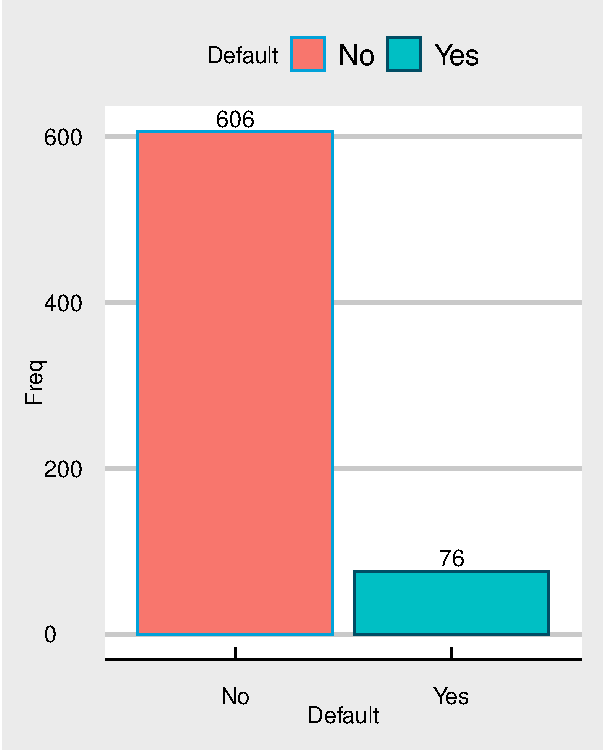
\includegraphics{DS-Report-20065124_files/figure-latex/FigureDefault-1} 

}

\caption{Binary Loan Defaults \label{FigureDefault}}\label{fig:FigureDefault}
\end{figure}

\hypertarget{features-and-target}{%
\subsubsection{Features and Target}\label{features-and-target}}

Now that there is a better understanding of the distribution of the
binary target variable indicating loan defaults, attention is turned to
the features. A few specific visualisations are displayed here that have
important implications to the analysis.

First, a tile plot is presented in Figure \ref{FigureLoanYear}. It shows
the loan status for loans that were granted in a particular year. All
the loans that were granted in 1998 are still running and an
overwhelming majority of them are not defaulted. This is likely due to
the fact that clients have not had much time to default on their loans
yet, rather than the fact that there is a particular characteristic
about loans granted in 1998 that make clients less likely to default on
payments. This is important, because a model will have to bear in mind
that loans granted recently are less likely to default currently, but
could skew out of sample predictions if the model attributes that to a
time trend in credit behaviour.

\begin{figure}[H]

{\centering 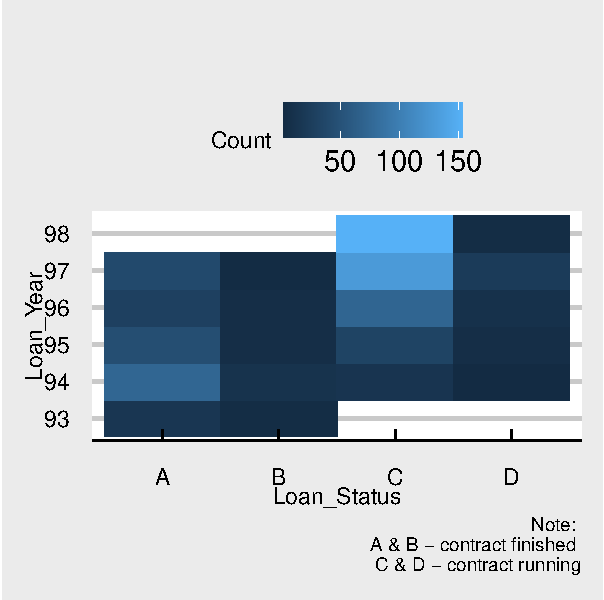
\includegraphics{DS-Report-20065124_files/figure-latex/FigureLoanYear-1} 

}

\caption{Loan Status By Year Loan Was Granted  \label{FigureLoanYear}}\label{fig:FigureLoanYear}
\end{figure}

Second, the some correlations between features are investigated. Figure
\ref{FigureCorrUnemploy} shows high correlation between district
unemployment in 1995 an 1996 and similarly Figure \ref{FigureCorrCrime}
shows high correlation between district crime figures in 1995 and 1996.
This is because crime and unemployment rate are slow to change in
successive years. This high correlation would be an issue for approaches
that struggle to deal with high multicollinearity. A solution to this
issue could be to create two indices (one for unemployment and one for
crime) using principal component analysis and only including that index.
However, because the correlations are so strong, only one of each
variable will be included in the data set because it would capture all
the relevant information, making the additional variables redundant.

\begin{figure}[H]

{\centering 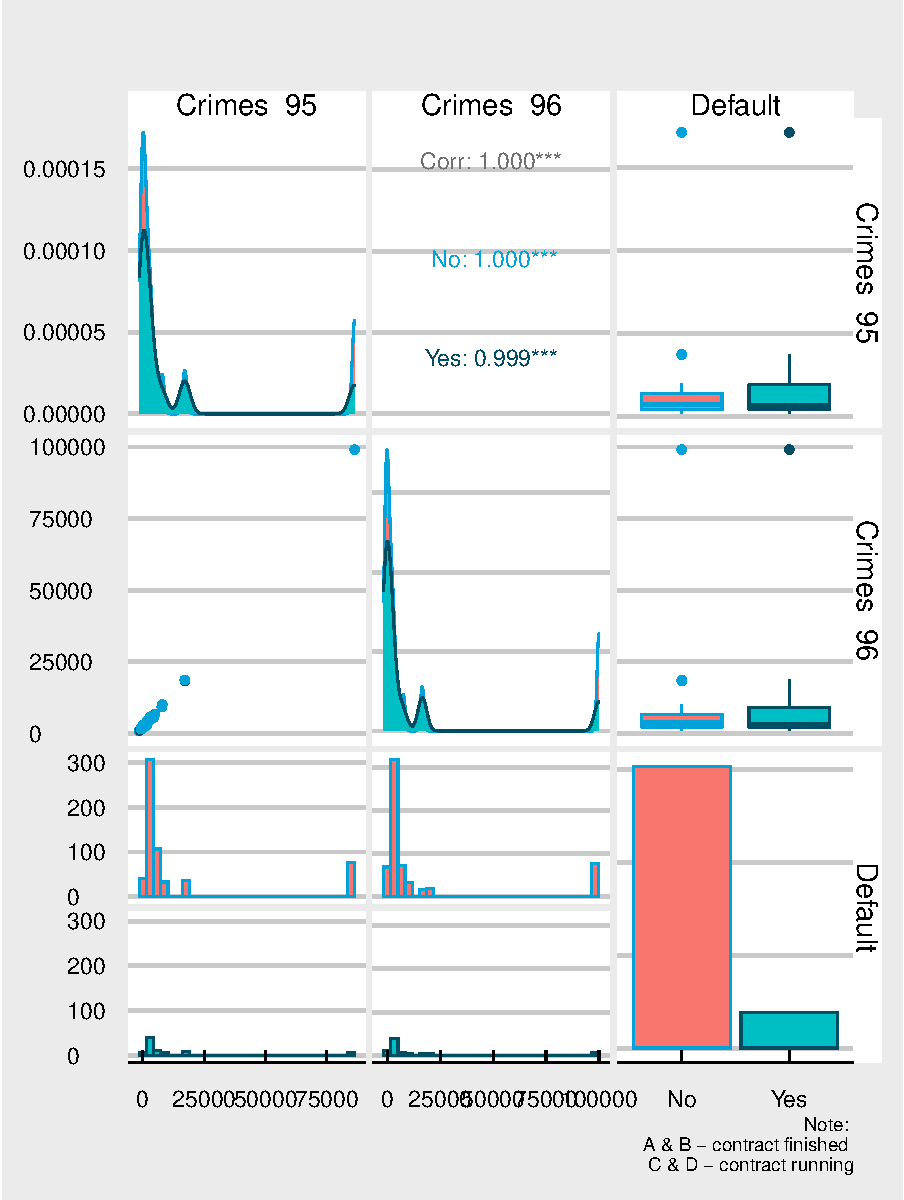
\includegraphics{DS-Report-20065124_files/figure-latex/FigureCorrCrime-1} 

}

\caption{Correlation Between Unemployment in 1995 and 1996  \label{FigureCrime}}\label{fig:FigureCorrCrime}
\end{figure}

\begin{figure}[H]

{\centering 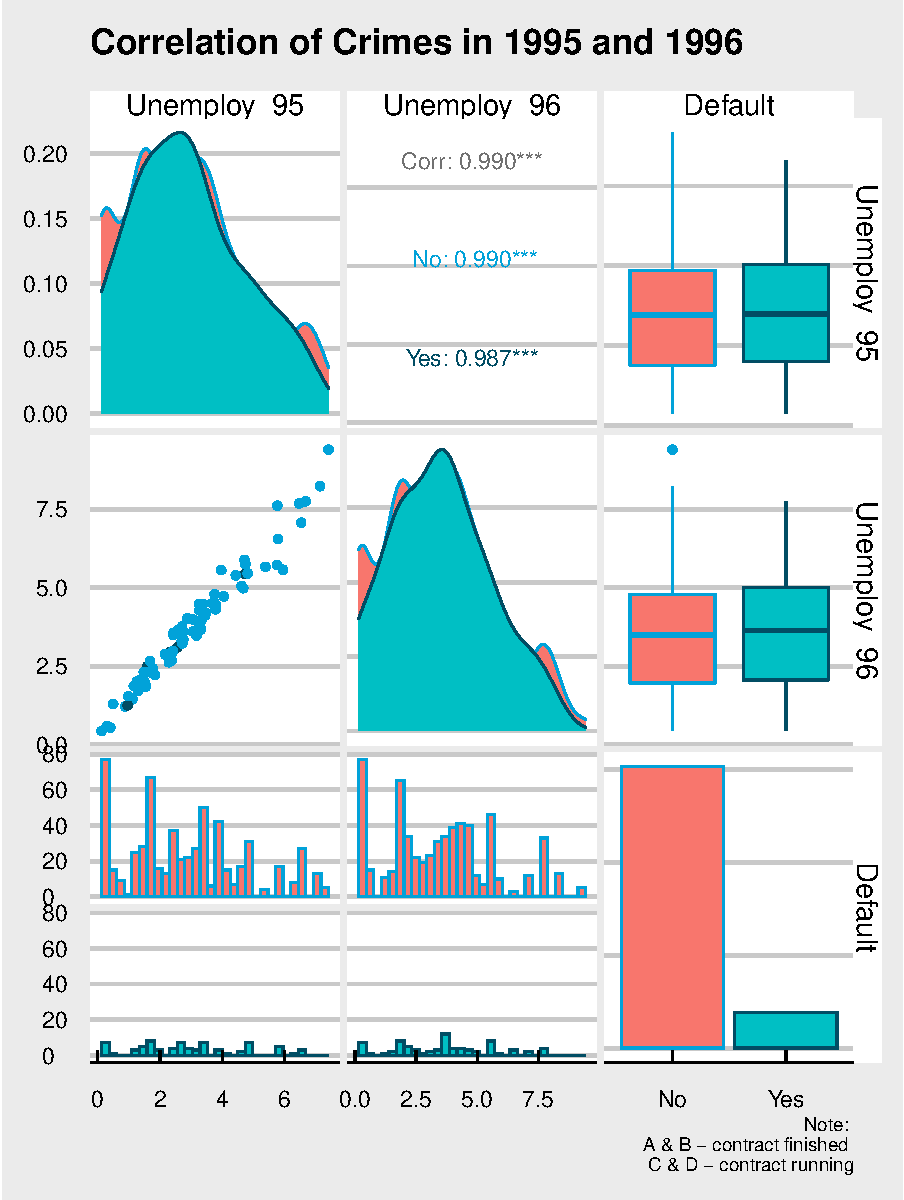
\includegraphics{DS-Report-20065124_files/figure-latex/FigureCorrUnemploy-1} 

}

\caption{Correlation Between Unemployment in 1995 and 1996  \label{FigureUnemploy}}\label{fig:FigureCorrUnemploy}
\end{figure}

Check near-zero variances of variables:

Two more variables are removed because they are found to have zero
variances. These are \emph{Present\_Day} and \emph{Owner}.
\emph{Present\_Day} has zero-variance by construction, and it was only
included to create the time since loan variable. Variables with no
variance are uninformative and are therefore excluded.

\hypertarget{final-features}{%
\subsection{Final Features}\label{final-features}}

There are a few missing values in this data set. Not all the methods
used in this report can handle missing values \textemdash specifically
the logistic regression models from packages \texttt{glm} and
\texttt{glmnet}. However, there are only 16 missing values in the full
data set, resulting 8 rows that have missing values. These rows will be
omitted. The effect of this omission should be negligible because a very
small proportion (0.012) of rows are omitted.

\newpage

\begin{longtable}{rll}
  \hline
 & VariableNames & VariableDescription \\ 
  \hline
1 & Default & Loan Default: No (0) or Yes (1) - Target Variable \\ 
  2 & Loan\_Amount & Loan Amount \\ 
  3 & Loan\_Duration & Duration Of The Loan Agreement \\ 
  4 & Loan\_Payments & Size Of Regular Loan Repayments \\ 
  5 & Loan\_Year & Year That Loan Contract Commenced \\ 
  6 & Loan\_Month & Month That Loan Contract Commenced \\ 
  7 & Account\_Year & Year In Which Account Was Created \\ 
  8 & Account\_Month & Month In Which Account Was Created \\ 
  9 & Issuance\_Freq & Frequency With Which Statements Are Issued \\ 
  10 & Age & Client Age \\ 
  11 & Gender & Client Gender \\ 
  12 & District\_Name & Name Of District In Which Client Resides \\ 
  13 & Region & Region In Which Client Resides \\ 
  14 & Inhabitants & District Population Size \\ 
  15 & VSmall\_Municipalities & Number Of Municipalities In District With Inhabitants $<$ 499 \\ 
  16 & Small\_Municipalities & Number Of Municipalities In District With Inhabitants 500 - 1 999 \\ 
  17 & Medium\_Municipalities & Number Of Municipalities In District With Inhabitants 2 000 - 9 999 \\ 
  18 & Big\_Municipalities & Number Of Municipalities In District With Inhabitants $>$ 10 000 \\ 
  19 & Cities & Number Of Cities In District \\ 
  20 & Urban\_Ratio & Ratio of Urban Inhabitants In District \\ 
  21 & Salary\_Ave & Average Salary In District \\ 
  22 & Unemploy\_95 & District Unemployment Rate In 1995 \\ 
  23 & Entrep & Number Of Entrpreneurs Per 1 000 Inhabitants In District \\ 
  24 & Crimes\_95 & Number Of Crimes Committed In 1995 \\ 
  25 & Mean\_Debited\_Order\_Amount & Mean Amount Debited Account \\ 
  26 & Modal\_Order\_Type & Most Frequent Payment Type (e.g. Insurance, etc.) By Account \\ 
  27 & Trans\_Credit & Number Of Credit Transactions Per Account \\ 
  28 & Transaction\_Freq & Amount Of Transactions Made By A Single Account \\ 
  29 & Trans\_Withdraw & Number Of Withdrawal Transactions Per Account \\ 
  30 & Trans\_Amount\_Mean & Mean Transaction Amount Per Account \\ 
  31 & Trans\_Balance & Mean BalancE In Account After A Transaction \\ 
  32 & Trans\_Mode & Modal Transaction Type (e.g. Credit Card Withdrawal, etc.) \\ 
  33 & Spread & Amount After Transaction minus the Mean Transaction Amount \\ 
   \hline
\hline
\caption{Variable Names and Descriptions \label{VariableTable}} 
\end{longtable}

\hypertarget{modeling}{%
\section{Modeling}\label{modeling}}

After the data has been wrangled and explored, the modeling can
commence. This section relies on the decisions and intuition developed
in section \ref{Data}. The need for resampling methods for model
assessment as well as the decision to use cross-validation for model
selection is briefly discussed. Thereafter, the logistic regression,
XGBoost, and causal forest models and their results are presented and
discussed.

\hypertarget{resampling}{%
\subsection{Resampling}\label{resampling}}

After data wrangling, the data set has 674 rows and 32 features.
Unfortunately this is not a data rich environment where there is enough
data to do a training, validation, and test split to select and assess
models, particularly in the case where there are multiple classes of
models \protect\hyperlink{ref-ESL}{Friedman, Hastie \& Tibshirani}
(\protect\hyperlink{ref-ESL}{2009}). Therefore, it is necessary to use a
resampling method.

While a training-test split is made here so that the final model can be
assessed on the independent test set, the model selection is done
through cross-validation on the training set. Cross-validation generally
has lower bias but higher variance than bootstrapping, which would be an
alternative resampling method for model selection and assessment.
Bootstrap can have especially high bias for small samples
\protect\hyperlink{ref-Efron}{Efron \& Tibshirani}
(\protect\hyperlink{ref-Efron}{1986}). CV estimates expected
generalization error rather than the generalizatio error, as shown by
simulation study in \protect\hyperlink{ref-ESL}{Friedman, Hastie \&
Tibshirani} (\protect\hyperlink{ref-ESL}{2009}). The expected
generalization error assesses the class of model rather than the
specific model trained on the given training data. Therefore, it is
appropriate for selecting model classes here. It is also used for
hyperparameter tuning.

\hypertarget{model-selection-and-assessment-strategy}{%
\subsection{Model Selection and Assessment
Strategy}\label{model-selection-and-assessment-strategy}}

\hypertarget{data-splits}{%
\subsubsection{Data Splits}\label{data-splits}}

This project considers multiple classes of models in order to find the
optimal model for prediction. Therefore, the model selection strategy
needs to a) select the optimal model for each class, b) select the
optimal model across classes. Thereafter, the optimal model needs to be
assessed by estimating the generalisation error. There are, however,
data constraints in trying to achieve this goal. The final clean data
set has 674 rows and 32 features. As we are not operating in a data-rich
environment, resampling strategies are employed to select models and
tune hyperparameters.

The process employed is as follows. The entire data set,
\(\mathcal{T}\), with 674 observations is split into a training and test
set, denoted \(\mathcal{T}_{tr}\) and \(\mathcal{T}_{te}\) respectively.
The training set, \(\mathcal{T}_{tr}\), comprises on 75\% of the
observations in \(\mathcal{T}\) such that it has a total of 506
observations. On the other hand, the test set has 168 and is kept aside
until the final estimated model has been attained so that it can be
assessed independently. Because there is a class imbalance in the
response variable as seen in Figure \ref{FigureDefault} where only
0.10979\% of loans are defaults , stratified sampling is used to ensure
that the distribution of the response in the test set resembles that in
the training set. The R package \emph{rsample} is used to conduct the
stratified training and test split. The resulting distributions of the
binary target variable, \emph{Default}, in
\(\mathcal{T}, \mathcal{T}_{tr}\), and \(\mathcal{T}_{te}\) can be seen
in Table \ref{DistributionDefaultTable}. These are fairly similar which
means gives confidence that the estimate of the generalisation error
attained from the test set will be reliable.

\begin{longtable}{rlll}
  \hline
 & Data & No & Yes \\ 
  \hline
1 & Full Data Set & 0.89021 & 0.10979 \\ 
  2 & Training Set & 0.89109 & 0.10891 \\ 
  3 & Test Set & 0.88757 & 0.11243 \\ 
   \hline
\hline
\caption{Comparing Distributions of Defaults in Different Data Sets \label{DistributionDefaultTable}} 
\end{longtable}

\hypertarget{cross-validation}{%
\subsubsection{Cross-Validation}\label{cross-validation}}

After the training-test split has been made, the \(\mathcal{T}_{te}\) is
set aside until the assessment of the final estimated model.
Cross-validation is used on the training set to select optimal models
within each model class through hyperparameter tuning, and to assess
which class of models is optimal for this particular classification
problem. Cross-validation is used rather than using a validation
approach \textemdash where \(\mathcal{T}_{tr}\) is split further into a
training set and a validation set \textemdash because using a single
validation set has high variance in cases where there is not an
abundance of data (\protect\hyperlink{ref-Molinaro}{Molinaro, Simon \&
Pfeiffer} (\protect\hyperlink{ref-Molinaro}{2005})).

In this analysis, 10-fold cross-validation is used. This is a common
choice in the literature \protect\hyperlink{ref-ESL}{Friedman, Hastie \&
Tibshirani} (\protect\hyperlink{ref-ESL}{2009}), and is appropriate here
because a larger number of folds means that the model will be trained on
more data each time which is important here because the data set is not
very large. However, 10-fold cross-validation is chosen ahead of an
alternative with an even larger number of folds \textemdash e.g.~LOOCV
\textemdash because when the number of folds becomes too large the
variance increases. For example, LOOCV estimates tend to have a large
variance because all the training sets are so similar
\protect\hyperlink{ref-ESL}{Friedman, Hastie \& Tibshirani}
(\protect\hyperlink{ref-ESL}{2009}). Weighing up these considerations
makes 10-fold cross-validation an appropriate choice for estimation of
the expected generalisation error and model selection. Moreover,
\protect\hyperlink{ref-Molinaro}{Molinaro, Simon \& Pfeiffer}
(\protect\hyperlink{ref-Molinaro}{2005}) suggests that 10-fold
cross-validation performs similarly to LOOCV yet is less computationally
expensive, further advocating for the use of 10-fold cross-validation in
this case. However, this time the data is not stratified before
splitting it into the 10 folds because using simple random sampling
should result in the effect of discrepancies in the distributions of
\emph{Default} canceling out over a large number of folds. Also note
that different folds are used for each model.

\hypertarget{logistic-regression}{%
\subsection{Logistic Regression}\label{logistic-regression}}

The first class of models used for classification is \emph{logistic
regression}. Logistic regression often provides a good benchmark for
classification problems because it can perform fairly well even though
it is a relatively simple approach. It is also frequently used in credit
risk screening to assess the risk of loan defaults, as is being done
here \protect\hyperlink{ref-ESL}{Friedman, Hastie \& Tibshirani}
(\protect\hyperlink{ref-ESL}{2009: 299}). Linear Logistic regression
could struggle with high correlation between features
(multicollinearity) such as that from Unemployment and Crime in 1995 and
1996, which is one of the reasons these variables were removed in
section \ref{Data}.

In this section, logistic regression models in 3 different ways: 1)
using all features, 2) using principal component analysis for dimension
reduction, 3) regularisation through imposing the L1 complexity penalty,
i.e.~LASSO, which reduces flexibility and is resistant to uninformative
features \protect\hyperlink{ref-ESL}{Friedman, Hastie \& Tibshirani}
(\protect\hyperlink{ref-ESL}{2009}). Two versions of the penalized
logistic regression is then presented, namely the tuned model minimising
the objective function as well as the model selected using the
one-standard-error rule. These three different approaches are used
because the data set has 32 features, which could result in overfitting
if the entire feature space is used in modeling. Because one cannot be
sure which features are appropriate to include in the model \emph{a
priori}, a data driven approach is used. The 10-fold cross-validation
error will suggest which approach has the highest prediction accuracy.
Here the \texttt{glm} package is used to fit the first two multiple
logistic regression models and the \texttt{glmnet} package is used for
the penalized logistic regression.

For the standard unpenalised multiple logistic regression models, there
is no hyperparameter tuning required. Figure \ref{FigureLogistic} shows
the misclassification error rate attained by doing 10-fold CV on the
penalized logistic regression. The two vertical dashed lines indicate
the optimal model as well as the model selected when using the
one-standard error rule. The misclassification rates showing in Figure
\ref{FigureLogistic} gives the average proportion of misclassified
observations in the validation fold. Results from the three selected
logistic regression models are given in Table \ref{LogisticTable}, along
with the results from the one-standard error rule model. These show that
while the standard multiple logistic regression does not perform too
poorly, and the PCA model improves slightly on it, regularization
substantially improves prediction accuracy. This suggests that there is
overfitting in the first two models, which is why the complexity penalty
that reduces variance improves the fit, even though it introduces some
bias in the model. The

\begin{figure}[H]

{\centering 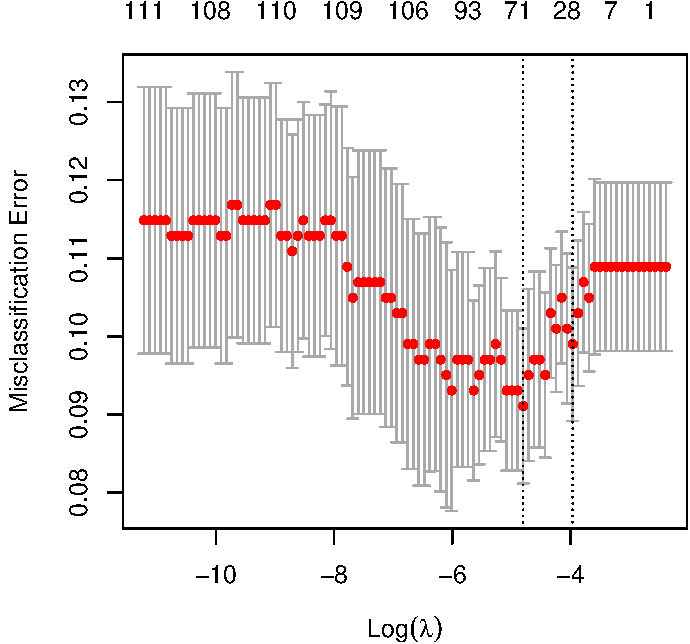
\includegraphics{DS-Report-20065124_files/figure-latex/unnamed-chunk-13-1} 

}

\caption{Misclassification Error of Penalised Logistic Regression for Different Penalties \label{FigureLogistic}}\label{fig:unnamed-chunk-13}
\end{figure}

\begin{longtable}{rlrrr}
  \hline
 & Models & 10-Fold CV Accuracy & Accuracy Standard Error & Lambda Value \\ 
  \hline
1 & Full Model (All Features) & 0.81 & 0.09 & 0.00 \\ 
  2 & PCA Model (Reduced Dimension) & 0.83 & 0.09 & 0.00 \\ 
  3 & L1 Regularized Model - Optimal & 0.91 & 0.01 & 0.01 \\ 
  4 & L1 Regularized Model - 1 S.E. Rule & 0.90 & 0.10 & 0.02 \\ 
   \hline
\hline
\caption{Comparing Logistic Regression Models for Model Selection \label{LogisticTable}} 
\end{longtable}

\hypertarget{extreme-gradient-boosting-machines}{%
\subsection{eXtreme Gradient Boosting
Machines}\label{extreme-gradient-boosting-machines}}

Gradient Boosting Machines very popular machine learning approaches that
tend to be successful in a variety of applications. These are ensemble
methods not dissimilar to bagging and random forests, although with some
alterations. Bagging and random forests are ensemble methods that
combine models and aggregate across the predictions generated by these
models. This can be done by taking some mean of the prediction, taking
the mode for either classification or regression, etc. Aggregating
across models decreases variance, so these ensemble methods are best
applied to models that naturally have high variance and low bias, such
as an overgrown decision tree \protect\hyperlink{ref-ESL}{Friedman,
Hastie \& Tibshirani} (\protect\hyperlink{ref-ESL}{2009}).

Boosting, however, works better in cases of high bias and low variance.
Here, an ensemble of shallow trees are grown that have low variance and
higher bias. Shallow trees are naturally weak learners. The boosting
methodology trains these weaker learners sequentially (rather than in
parallel like in bagging) so that each successive tree improves on its
predecessor. Gradient boosting grows shallow trees in sequence, and fits
the new tree to the residuals at the previous step. It is called
\emph{gradient boosting} because it uses gradient descent to minimise
loss when new models are added in sequence.

The state-of-the-art package that is popularly used is eXtreme Gradient
Boosting (XGBoost), an implementation of Gradient Boosting that is
specifically designed to improve speed and performance. The sequential
training employed by gradient boosting algorithms are typically very
slow and therefore not scalable. The XGBoost library supports a number
of features that are extensions to gradient boosting machines. In this
report, the learning rate, stochastic descent through sub-sampling, and
regularization are all used to attempt to improve model performance.

There are three of these regularisation hyperparameters: 1. \(\gamma\) -
limits the depth of each tree by specifying the minimum loss reduction
required to induce a further split 2. \(\alpha\) - the L1 regularization
penalty 3. \(\lambda\) - the L2 regularization penalty where \(\alpha\)
and \(\lambda\) together determine how large the influence of the leaves
in a tree are. If both are larger than 0 then elastic net regularization
is performed. It is recommended to tune all three regularization
parameters \protect\hyperlink{ref-Boehmke}{Boehmke \& Greenwell}
(\protect\hyperlink{ref-Boehmke}{2019}).

\hypertarget{prepare-data}{%
\subsubsection{Prepare Data}\label{prepare-data}}

The \texttt{xgboost} package requires a matrix input for the features
and a vector for the target. Therefore, the data must all be encoded
numerically and converted into a matrix. All categorical features are
encoded using one-hot encoding.

\hypertarget{default-xgboost}{%
\subsubsection{Default XGBoost}\label{default-xgboost}}

The first model uses the default parameters that are specified in the
package documentation. The objective chosen is \emph{binary::logistic}
that specifies logistic regression for binary classification, giving
probabilities as output. The default hyperparameter values generally
perform fairly well \protect\hyperlink{ref-Boehmke}{Boehmke \&
Greenwell} (\protect\hyperlink{ref-Boehmke}{2019}), and will be compared
to the tuned models.

\hypertarget{partially-tuned-xgboost}{%
\subsubsection{Partially Tuned XGBoost}\label{partially-tuned-xgboost}}

For the second XGBoost model some regularization is introduced by tuning
the \(\gamma\), \(\lambda\), and \(\alpha\) hyperparameters. Also, the
number of iterations is also tuned. The other hyperparameters still
receive their default values. The hyperparameter tuning is done through
conducting a grid search for different values for the hyperparameters
and choosing the optimal ones. The maximum number of trees grown in
order to achieve those hyperparameters will then be selected as the
\texttt{nrounds} parameter, giving the maximum number of boosting
iterations.

\begin{longtable}{rrrrrr}
  \hline
 & eta & max\_depth & min\_child\_weight & subsample & colsample\_bytree \\ 
  \hline
1 & 0.30 & 6.00 & 3.00 & 1.00 & 1.00 \\ 
   \hline
\hline
\caption{Default Hyperparameters for XGBoost Partially Tuned Model \label{XGBTune1Table}} 
\end{longtable}
\begin{longtable}{rrrrrrr}
  \hline
 & gamma & lambda & alpha & train\_error & test\_error & trees \\ 
  \hline
1 & 0.00 & 1.00 & 0.00 & 0.00 & 0.09 & 44.00 \\ 
  2 & 0.00 & 10.00 & 0.10 & 0.00 & 0.09 & 23.00 \\ 
  3 & 1.00 & 0.01 & 1.00 & 0.02 & 0.09 & 14.00 \\ 
  4 & 0.00 & 1.00 & 1.00 & 0.00 & 0.09 & 26.00 \\ 
  5 & 0.00 & 0.00 & 1.00 & 0.00 & 0.09 & 53.00 \\ 
  6 & 0.00 & 10.00 & 0.00 & 0.00 & 0.09 & 28.00 \\ 
  7 & 1.00 & 10.00 & 0.10 & 0.04 & 0.09 & 22.00 \\ 
  8 & 0.00 & 0.00 & 0.01 & 0.00 & 0.09 & 22.00 \\ 
  9 & 0.00 & 0.01 & 0.01 & 0.00 & 0.09 & 28.00 \\ 
  10 & 1.00 & 1.00 & 1.00 & 0.03 & 0.09 & 17.00 \\ 
   \hline
\hline
\caption{Tuning Regularization Hyperparameters for XGBoost Partially Tuned Model \label{XGBTune1Table_b}} 
\end{longtable}

\begin{verbatim}
## # A tibble: 10 x 11
##      eta max_depth min_child_weight subsample colsample_bytree gamma lambda
##    <dbl>     <dbl>            <dbl>     <dbl>            <dbl> <dbl>  <dbl>
##  1   0.3         6                3         1                1     0   1   
##  2   0.3         6                3         1                1     0  10   
##  3   0.3         6                3         1                1     1   0.01
##  4   0.3         6                3         1                1     0   1   
##  5   0.3         6                3         1                1     0   0   
##  6   0.3         6                3         1                1     0  10   
##  7   0.3         6                3         1                1     1  10   
##  8   0.3         6                3         1                1     0   0   
##  9   0.3         6                3         1                1     0   0.01
## 10   0.3         6                3         1                1     1   1   
## # ... with 4 more variables: alpha <dbl>, train_error <dbl>, test_error <dbl>,
## #   trees <dbl>
\end{verbatim}

The default hyperparameter values can be seen in Table
\ref{XGBTune1Table}. Table \ref{XGBTune1Table_b} shows that the tuned
hyperparameter values are \(\gamma\) = 0, \(\lambda\) = 1, and
\(\alpha\) = 0. This is attained after 44 iterations. The training error
for this tuned model is 0, showing that the model perfectly fits the
training data. This is the lowest training error, which is also attained
in rows 8 and 9 of Table \ref{XGBTune1Table_b}, which has hyperparameter
values of 0 and 0 for \(\gamma\), 0 and 0.01 for \(\lambda\), and 0.01
and 0.01 for \(\alpha\) respectively. However, the latter two models
have cross-validation errors of 0.09298 and 0.09298, while the optimal
model has a cross-validation error of 0.0871. The optimal model only
regularizes through the \(\lambda\) parameter meaning that it only
utilises the L2 regularization penalty. It also does not limit tree
depth through \(\gamma\), which suggests that some flexibility with
regards to tree depth improves prediction accuracy even though it
inevitably increases variance. The optimal model balances the
bias-variance trade-off to optimize prediction accuracy. Now train the
partially tuned model with the tuned regularization hyperparameters and
\texttt{nrounds} parameter, along with the default values for other
parameters.

\hypertarget{fully-tuned-xgboost-with-mlr}{%
\subsubsection{Fully Tuned XGBoost with
MLR}\label{fully-tuned-xgboost-with-mlr}}

The partially tuned XGBoost model trained above The package \texttt{mlr}
allows more convenient parameter tuning for the xgboost model. Now we
proceed with a random/grid search procedure to improve on prediction
accuracy. The default \texttt{nrounds} and \(\eta\) parameters are used
initially to simplify the procedure. While XGBoost is fast, the process
is sped up further by using a random search rather than a grid search
for the best parameters. In random search, 10 models are trained with
different parameters and the one with the lowest error is chosen. Time
improve the computation speed even further, a parallel backend is set up
to use all the cores in parallel. After tuning the parameters in Table
\ref{XGBTune1Table} that were previously chosen as defaults, the grid
search is again employed to tune the regularisation and \texttt{nrounds}
parameters. The tuned hyperparameters that were previously defaults can
be found in Table \ref{XGBTune2Table_b} while the grid search for the
regularization parameters produces Table \ref{XGBTune2Table_b}.

\begin{longtable}{rrrrrr}
  \hline
 & eta & max\_depth & min\_child\_weight & subsample & colsample\_bytree \\ 
  \hline
1 & 0.30 & 7.00 & 7.35 & 0.98 & 0.51 \\ 
   \hline
\hline
\caption{Tuning Previous Default Hyperparameters for XGBoost Fully Tuned Model \label{XGBTune2Table}} 
\end{longtable}

\newpage
\begin{longtable}{rrrrrrr}
  \hline
 & gamma & lambda & alpha & train\_error & test\_error & trees \\ 
  \hline
1 & 0.00 & 0.01 & 0.01 & 0.02 & 0.09 & 94.00 \\ 
  2 & 0.00 & 0.00 & 0.01 & 0.02 & 0.09 & 91.00 \\ 
  3 & 0.00 & 0.01 & 0.00 & 0.02 & 0.09 & 91.00 \\ 
  4 & 0.00 & 0.10 & 0.00 & 0.02 & 0.09 & 94.00 \\ 
  5 & 0.00 & 0.10 & 0.10 & 0.02 & 0.09 & 111.00 \\ 
  6 & 0.00 & 1.00 & 0.00 & 0.02 & 0.09 & 90.00 \\ 
  7 & 0.00 & 1.00 & 1.00 & 0.03 & 0.09 & 105.00 \\ 
  8 & 0.00 & 1.00 & 0.01 & 0.02 & 0.09 & 102.00 \\ 
  9 & 0.00 & 0.00 & 0.00 & 0.02 & 0.09 & 94.00 \\ 
  10 & 0.00 & 0.10 & 0.01 & 0.02 & 0.09 & 72.00 \\ 
   \hline
\hline
\caption{Tuning Regularization Hyperparameters for XGBoost Fully Tuned Model \label{XGBTune2Table_b}} 
\end{longtable}

\hypertarget{final-model-assessment}{%
\section{Final Model Assessment}\label{final-model-assessment}}

In this section the final XGBoost model is trained on the full training
data and assessed on the test set. Before giving the test error, a
variable importance plot can be seen in Figure \ref{FigureVIP}. It shows
that Spread, the mean transaction amount, and the account balance after
some transaction are the most important variables in determining splits,
and therefore prediction.

\begin{figure}[H]

{\centering 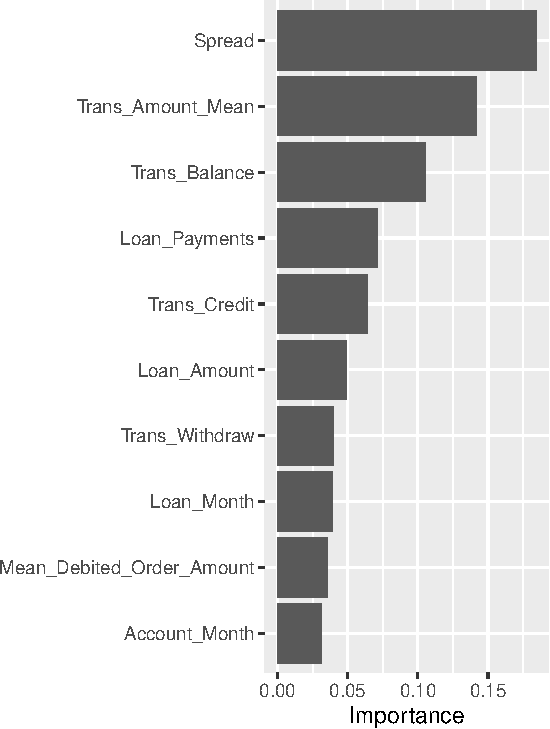
\includegraphics{DS-Report-20065124_files/figure-latex/unnamed-chunk-35-1} 

}

\caption{Variable Importance \label{FigureVIP}}\label{fig:unnamed-chunk-35}
\end{figure}

The final estimated test error of the fully tuned XGBoost model is
0.8934911. This is only slightly less than the estimated error by
cross-validation. However, it is also less than the CV-error of the
penalized logistic regression. Therefore, the penalized logistic
regression remains a very good option for credit risk screening,
especially because it is not nearly as complex as XGBoost.

\hypertarget{entrepreneurs-and-risky-loans}{%
\section{Entrepreneurs and Risky
Loans}\label{entrepreneurs-and-risky-loans}}

Entrepreneurs require access to credit as a source of capital in order
to finance business ventures. However, banks also face the risk that the
entrepreneur is unsuccessful and will therefore default on the loan
repayment. Entrepreneurs tend to be more open to taking risks, often not
even requiring a risk premium to induce them to invest in risky projects
\protect\hyperlink{ref-Risk}{Vereshchagina \& Hopenhayn}
(\protect\hyperlink{ref-Risk}{2009}). The density of entrepreneurs in a
district may therefore have an causal effect on the probability of loan
default that could be important for banks to consider. Importantly, the
differences between groups of entrepreneurs in Czech is known to be
influential in determining their behaviour
\protect\hyperlink{ref-Entrep}{Ključnikov \& Belás}
(\protect\hyperlink{ref-Entrep}{2016}).

This section of the analysis investigates the relationship between loan
defaults and the number of entrepreneurs per 1 000 inhabitants in a
district. To build off the tree-based ensemble approach used with
XGBoost, a causal forest procedure is utilised to estimate the causal
effect of the density of entrepreneurs in a district on loan defaults.
Causal forests are a generalisation of the random forest by
\protect\hyperlink{ref-Breiman2001}{Breiman}
(\protect\hyperlink{ref-Breiman2001}{2001}). However, rather than merely
splitting on variables to minimise the root mean squared error, the
objective of the causal forest is to maximise treatment heterogeneity
between nodes. Therefore, variables that create heterogenous treatment
effects are favoured for splits while variables that increase the
variance of the treatment effect are penalised
\protect\hyperlink{ref-AtheyImbensRecursive}{Athey \& Imbens}
(\protect\hyperlink{ref-AtheyImbensRecursive}{2016}).

The causal forest approach developed by
\protect\hyperlink{ref-AtheyASA2018}{Wager \& Athey}
(\protect\hyperlink{ref-AtheyASA2018}{2018}) and
\protect\hyperlink{ref-AtheyGRF2019}{Athey, Tibshirani \& Wager}
(\protect\hyperlink{ref-AtheyGRF2019}{2019}) is appropriate in
estimating the causal effect of entrepreneurs on loan default rates
because of the likely heterogeneity
\protect\hyperlink{ref-Entrep}{Ključnikov \& Belás}
(\protect\hyperlink{ref-Entrep}{2016}) and non-linear, unknown
interactions in treatment effects that more traditional econometric
methods are not as adept at dealing with
\protect\hyperlink{ref-StateOfEconometrics}{Athey \& Imbens}
(\protect\hyperlink{ref-StateOfEconometrics}{2017}). The causal forest
is specifically designed to estimate conditional average treatment
effects in highly non-linear environments where there is potential
heterogeneity in treatment effects. In this sense, it leverages the
flexibility that machine learning algorithms afford. The strongest
assumption that is made is that there are no unobservable confounding
factors within nodes that would bias estimates. While this assumption is
fairly strong, it is not as strong as the unconfoundedness assumption in
standard econometrics because of the ability for the algorithm to
provide more intricate covariate combinations
\protect\hyperlink{ref-AtheyASA2018}{Wager \& Athey}
(\protect\hyperlink{ref-AtheyASA2018}{2018}). Even if this assumption is
violated, however, the conditional average treatment effects are still
highly informative for the Czech bank, even if interpretations are not
strictly causal.

In this analysis, I closely follow the estimation procedure of
\protect\hyperlink{ref-Athey2019Application}{Athey \& Wager}
(\protect\hyperlink{ref-Athey2019Application}{2019}). To prepare the
data for the causal forest, everything again needs to be numerically
encoded and stored in a matrix.
\protect\hyperlink{ref-Athey2019Application}{Athey \& Wager}
(\protect\hyperlink{ref-Athey2019Application}{2019}) present an
algorithm for estimating treatment effects with causal forests. First,
random forests are used to predict both the response, \(Default\), and
the treatment, \(Entrepreneur\), using the features as inputs. This
orthogonalises the procedure, making estimates more robust to the effect
of confounders. These predictions are then used as inputs to the causal
forest, along with the true values. As recommended by
\protect\hyperlink{ref-Athey2019Application}{Athey \& Wager}
(\protect\hyperlink{ref-Athey2019Application}{2019}), I tune all
hyperparameters using cross-validation, excluding the decision to set
the number of trees as 10 000. This is done to allow appropriate
estimation of standard errors due to the convenient asymptotic
properties of causal forests \protect\hyperlink{ref-AtheyASA2018}{Wager
\& Athey} (\protect\hyperlink{ref-AtheyASA2018}{2018}). This entire
procedure is performed on the training data.

\begin{table}[H]
\centering
\begin{tabular}{rlr}
  \hline
 & Variable & VariableImportance \\ 
  \hline
1 & Loan\_Amount & 0.08 \\ 
  2 & Loan\_Duration & 0.01 \\ 
  3 & Loan\_Payments & 0.18 \\ 
  4 & Loan\_Year & 0.01 \\ 
  5 & Loan\_Month & 0.03 \\ 
  6 & Account\_Year & 0.00 \\ 
  7 & Account\_Month & 0.03 \\ 
  8 & Issuance\_Freq & 0.00 \\ 
  9 & Age & 0.03 \\ 
  10 & Gender & 0.00 \\ 
  11 & District\_Name & 0.05 \\ 
  12 & Region & 0.02 \\ 
  13 & Inhabitants & 0.02 \\ 
  14 & VSmall\_Municipalities & 0.03 \\ 
  15 & Small\_Municipalities & 0.01 \\ 
  16 & Medium\_Municipalities & 0.01 \\ 
  17 & Big\_Municipalities & 0.01 \\ 
  18 & Cities & 0.02 \\ 
  19 & Urban\_Ratio & 0.01 \\ 
  20 & Salary\_Ave & 0.05 \\ 
  21 & Unemploy\_95 & 0.03 \\ 
  22 & Entrep & 0.08 \\ 
  23 & Crimes\_95 & 0.02 \\ 
  24 & Mean\_Debited\_Order\_Amount & 0.05 \\ 
  25 & Modal\_Order\_Type & 0.00 \\ 
  26 & Trans\_Credit & 0.02 \\ 
  27 & Transaction\_Freq & 0.02 \\ 
  28 & Trans\_Withdraw & 0.02 \\ 
  29 & Trans\_Amount\_Mean & 0.05 \\ 
  30 & Trans\_Balance & 0.05 \\ 
  31 & Trans\_Mode & 0.00 \\ 
  32 & Spread & 0.06 \\ 
   \hline
\end{tabular}
\caption{Variable Importance for Causal Forest \label{VarImpCForest}} 
\end{table}

\begin{figure}[H]

{\centering 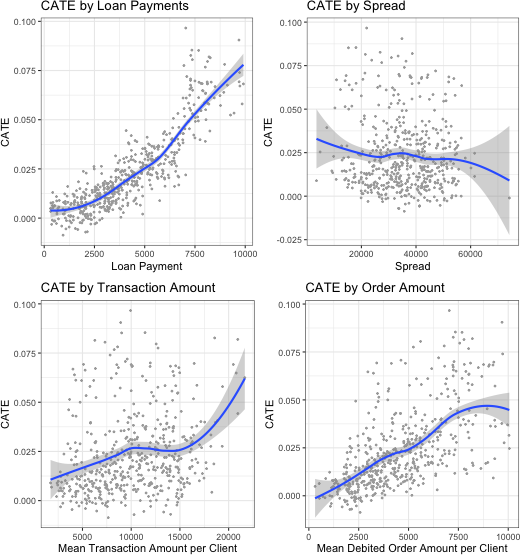
\includegraphics{DS-Report-20065124_files/figure-latex/FigureCATE-1} 

}

\caption{Conditional Average Treatment Effects (CATE) for 4 Important Variables \label{FigureCATE}}\label{fig:FigureCATE}
\end{figure}

The average partial effect and confidence interval estimated in
0.0617487, 0.0254175. Figure \ref{FigureCATE} shows the average
treatment effects of the density of entrepreneurs on loan defaults
conditional on four of the most important variables, as indicated by
variable importance measures in Table \ref{VarImpCForest}. Figure
\ref{FigureCATE} gives evidence of the extent of heterogeneity and
non-linearity in the effect of entrepreneurs on loan defaults. While a
large amount of entrepreneurs in a district unambiguously increase loan
default rates, the magnitude of that effect is highly variable. A high
density of entrepreneurs has a far more substantial impact on the loan
defaults of clients with high loan repayment amounts. Similarly, clients
with high average transaction amounts are also most affected by the
ubiquity of entrepreneurs. On the other hand, the effect of
entrepreneurs on loan defaults remains fairly stable as spread
increases. Therefore, banks should closely monitor the credit worthiness
of clients from districts with many entrepreneurs when those clients
have high average transaction amounts or large regular loan repayments.

\hypertarget{conclusion-and-recommendations}{%
\section{Conclusion and
Recommendations}\label{conclusion-and-recommendations}}

The complex fully tuned XGBoost model and the penalised logistic
regression model have very similar performance. It may be best to go
with the simpler model, even though XGBoost is generally a good option
for prediction. It is also of value to banks to know that a high density
of entrepreneurs increases their credit risk and that there is
substantial heterogeneity in this effect. There is, however, more
investigation that should go into this effect.

\newpage

\hypertarget{references}{%
\section*{References}\label{references}}
\addcontentsline{toc}{section}{References}

\hypertarget{refs}{}
\begin{CSLReferences}{1}{0}
\leavevmode\hypertarget{ref-AtheyImbensRecursive}{}%
Athey, S. \& Imbens, G. 2016. Recursive partitioning for heterogeneous
causal effects. \emph{Proceedings of the National Academy of Sciences}.
113(27):7353--7360.

\leavevmode\hypertarget{ref-StateOfEconometrics}{}%
Athey, S. \& Imbens, G.W. 2017. The state of applied econometrics:
Causality and policy evaluation. \emph{Journal of Economic
Perspectives}. 31(2):3--32.

\leavevmode\hypertarget{ref-Athey2019Application}{}%
Athey, S. \& Wager, S. 2019. Estimating treatment effects with causal
forests: An application. \emph{arXiv preprint arXiv:1902.07409}.

\leavevmode\hypertarget{ref-AtheyGRF2019}{}%
Athey, S., Tibshirani, J. \& Wager, S. 2019. Generalized random forests.
\emph{Annals of Statistics}. 47(2):1148--1178.

\leavevmode\hypertarget{ref-Data}{}%
Berka, P. 1999. {Workshop notes on Discovery Challenge PKDD'99}.
{[}Online{]}, Available: \url{http://lisp.vse.cz/pkdd99/}.

\leavevmode\hypertarget{ref-Boehmke}{}%
Boehmke, B. \& Greenwell, B.M. 2019. \emph{Hands-on machine learning
with r}. CRC Press.

\leavevmode\hypertarget{ref-Breiman2001}{}%
Breiman, L. 2001. Random forests. \emph{Machine learning}. 45(1):5--32.

\leavevmode\hypertarget{ref-Efron}{}%
Efron, B. \& Tibshirani, R. 1986. Bootstrap methods for standard errors,
confidence intervals, and other measures of statistical accuracy.
\emph{Statistical science}. 54--75.

\leavevmode\hypertarget{ref-ESL}{}%
Friedman, J., Hastie, T. \& Tibshirani, R. 2009. \emph{The elements of
statistical learning}. 2nd ed. Vol. 1. (10). Springer series in
statistics New York.

\leavevmode\hypertarget{ref-Entrep}{}%
Ključnikov, A. \& Belás, J. 2016. Approaches of czech entrepreneurs to
debt financing and management of credit risk.
\emph{Equilibrium-Quarterly Journal of Economics and Economic Policy}.

\leavevmode\hypertarget{ref-Molinaro}{}%
Molinaro, A.M., Simon, R. \& Pfeiffer, R.M. 2005. Prediction error
estimation: A comparison of resampling methods. \emph{Bioinformatics}.
21(15):3301--3307.

\leavevmode\hypertarget{ref-Risk}{}%
Vereshchagina, G. \& Hopenhayn, H.A. 2009. Risk taking by entrepreneurs.
\emph{American Economic Review}. 99(5):1808--30.

\leavevmode\hypertarget{ref-AtheyASA2018}{}%
Wager, S. \& Athey, S. 2018. Estimation and inference of heterogeneous
treatment effects using random forests. \emph{Journal of the American
Statistical Association}. 113(523):1228--1242.

\end{CSLReferences}

\hypertarget{appendix}{%
\section*{Appendix}\label{appendix}}
\addcontentsline{toc}{section}{Appendix}

\hypertarget{appendix-a}{%
\subsection*{Appendix A}\label{appendix-a}}
\addcontentsline{toc}{subsection}{Appendix A}

Some appendix information here

\hypertarget{appendix-b}{%
\subsection*{Appendix B}\label{appendix-b}}
\addcontentsline{toc}{subsection}{Appendix B}

\bibliography{Tex/ref}





\end{document}
